% -*- coding: utf-8 -*-
%%!TEX encoding = UTF-8 Unicode 

\newpage

    %%\part{ANEXOS}
    
    %%\newpage
    
    \appendix
    
    \clearpage % o \cleardoublepage
    \addappheadtotoc
    \appendixpage

    %\begin{center}
    %{\Large\bf Apéndice A: }
    %\phantomsection
    %\addcontentsline{toc}{section}{Apéndice A: Instalación} 
    %\end{center}
    %\label{chap:configurationchapter}
    
    \chapter{Apéndice A: Instalación y ejecución}
    
    La instalación de \emph{FreeStation} esta compuesta por dos instalaciones
    diferentes. La instalación del entorno servidor con \emph{Backend} PHP, Python y ZeroC ICE.
    
    \section{\uppercase{Instalación del entorno servidor}}
    
    \subsection{Instalación de Zero C ICE con repositorio}
    
    Esta opción de instalación es sencilla y cómoda, pero no esta aconsejada
    para desarrolladores que necesiten actualizaciones con bastante frecuencia o
    disponer de una versión determinada.

    Para proceder es necesario descargar el repositorios (en estos momentos
    para la versión más actual 3.4) desde la página web oficial:

    \begin{lstlisting}[language={bash}, texcl=true, caption={Añadir repositorio
    ICE}] sudo wget http://download.zeroc.com/Ice/3.4/rhel6/zeroc-ice-rhel6.repo
    -O /etc/yum.repos.d/zeroc-ice-rhel6.repo
    \end{lstlisting}
    
    Posteriormente se debe activar el repositorio e instalar el paquete ZeroC
    Ice y biblioteca Ice para Python:

    \begin{lstlisting}[language={bash}, texcl=false, caption={Instalación Zero
    C ICE desde repositorios}] sudo yum --enablerepo zeroc-ice install -y ice
    ice-python
    \end{lstlisting}

    \newpage
    
    \subsection{Instalación desde fuentes}
 
    Si la necesidad de uso esta más orientada al enfoque desarrollador, se puede
    compilar la versión que se requiera para desarrollo. En el momento de
    escribir el proyecto se compiló para la versión 3.4.2 de ICE.

    Como prerrequisito para la compilación es necesario instalar la biblioteca
    mcpp o ``portable C preprocessor'' desde el repo de ZeroC Ice (también
    se puede optar por bajar y compilar los fuentes de mcpp, pero no es
    necesario):

    \begin{lstlisting}[language={bash}, texcl=false, caption={Instalación mcpp}]
    sudo yum install -y mcpp-devel
    \end{lstlisting}

    A continuación, se descargan los ficheros fuente de Ice, se descomprimen y
    se compilan para la versión en C++ y su binding para Python (en este 
    caso para la versión 3.4.2 de Ice). Para ello puede realizarse todo en una
    línea con:
    
    \begin{lstlisting}[language={bash}, texcl=false, caption={Instalación Zero
    C ICE}] sudo wget http://zeroc.com/download/Ice/3.4/Ice-3.4.2.tar.gz; tar
    xvzf Ice-*.tar.gz; cd Ice-*/cpp; make; make install; cd ../py/; make;make install
    \end{lstlisting}

    La instalación de Ice quedará bajo /opt/Ice-3.4.2/ y el binding python sobre
    /opt/Ice-3.4.2/python. Es importante recalcar que el binding python se
    asociara con la versión de defecto de Python en el sistema si se dispone de
    varias.

    Por último, es necesario indicar el el PATH y el PYTHONPATH del sistema,
    donde se encuentra la instalación de Ice y su binding de Python:

    \begin{lstlisting}[language={bash}, texcl=false, caption={Configuración
    path}] sudo export PATH=/opt/Ice-3.4.2/bin:$PATH
    sudo export PYTHONPATH=/opt/Ice-3.4.2/python:$PYTHONPATH
    \end{lstlisting}

    \newpage
    
    \section{\uppercase{Instalación del entorno cliente}}
    
    La instalación del entorno cliente necesita de la biblioteca
    python-feedparser si se utiliza el widget \emph{FeedParser}. Para su
    instalación en entornos basados en Debian:
    
    \begin{lstlisting}[language={bash}, texcl=false, caption={Instalación
        python-feedparser}] sudo apt-get install python-feedparser
    \end{lstlisting}
    
    Para el widget VideoArea es necesaria la dependencia Gstreamer:
    \begin{lstlisting}[language={bash}, texcl=false, caption={Instalación
        dependencias Gstreamer}] sudo apt-get install gir1.2-gstreamer-1.0
        gstreamer-tools gstreamer1.0-alsa gstreamer1.0-libav gstreamer1.0-plugins-bad gstreamer1.0-plugins-base gstreamer1.0-plugins-good
    gstreamer1.0-plugins-ugly  gstreamer1.0-pulseaudio gstreamer1.0-tools
    gstreamer1.0-x libgstreamer-plugins-bad1.0-0 libgstreamer-plugins-base1.0-0
    libgstreamer1.0-0
    \end{lstlisting}
    
    Para widgets basados en CouchDB es necesario instalar couchdb y sus
    dependencias desde el PPA de Novacut:
    
    \begin{lstlisting}[language={bash}, texcl=false, caption={Añadir PPA daily
    Novacut}] sudo add-apt-repository ppa:novacut/daily && sudo apt-get
    update
    \end{lstlisting}
    
    Posteriormente se instalan los paquetes necesarios:
    
    \begin{lstlisting}[language={bash}, texcl=false, caption={Instalar paquetes
    del PPA de Novacut}] sudo apt-get install couchdb couchdb-bin microfiber
    novacut dmedia userwebkit
    \end{lstlisting}

    Para la ejecución del cliente ICE es necesaria la instalación del paquete
    zeroc-ice34 para soporte Zero C ICE y el paquete python-zeroc-ice para
    obtener el soporte del binding de ICE para python.

    En sistema basados en Debian, como Ubuntu, el comando de instalación es:

    \begin{lstlisting}[language={bash}, texcl=false, caption={Instalar
    dependencias ICE}] sudo apt-get install zeroc-ice34 python-zeroc-ice
    \end{lstlisting}

    Desafortunadamente, el cliente de \emph{FreeStation} para Ice no puede ejecutarse
    en Python 3 debido a que en el momento de escribir este proyecto de fin de
    carrera no existía una versión del binding
    adaptada\footnote{Zero C ICE soporte Python 3:
    \url{http://www.zeroc.com/forums/help-center/5138-support-python-3-x-scheduled.html}}.

    En su lugar el código debe ejecutarse con un intérprete basado en Python
    2.7.
    
    \section{\uppercase{Funcionamiento y ejecución}}

    \subsection{Ejecución de la interfaz cliente}
    \label{sec:clientexecution}
    
    Acceder a la carpeta FreeStation/freestation:
    
    \begin{lstlisting}[language={bash}, texcl=false, caption={Cambiar
    directorio}] cd FreeStation/freestation/
    \end{lstlisting}
    
    Posteriormente ejecutar el watchdog.py con un inteprete basado en Python 3:

    \begin{lstlisting}[language={bash}, texcl=false, caption={Ejecutar cliente}]
    python3 watchdog.py
    \end{lstlisting}

    Esto iniciara la interfaz del POI.
   
    \subsection{Ejecución del cliente basado en ICE}
    
    Usando un intérprete basado en Python 2.7, un ejemplo de ejecución 
    cuando el servidor no esta activo:

    \begin{lstlisting}[language={bash}, texcl=false, caption={Ejemplo de
    conexión rechazada}] python2.7 FreeStationClient.py 
    FreeStation Client 0.1
    Ice Version 3.4.2
    Base: Api -t:tcp -h 123.123.123.123 -p 10000 -t 60000:udp -p 0 -z
    Error: connection refused. Please, check if the server is running or you are connecting properly.
    Client abort.
    \end{lstlisting}

    Nota: La IP ha sido modificada con propósitos de privacidad.
    
    Cuando el servidor esta activo, pero el cliente no esta habilitado,
    producirá una salida diferente:
    
    \begin{lstlisting}[language={bash}, texcl=false, caption={Ejemplo de
    conexión no autorizada}] Ice Version 3.4.2
    Base: Api -t:tcp -h 123.123.123.123 -p 10000 -t 60000:udp -p 0 -z
    Proxy: Api -t:tcp -h 123.123.123.123 -p 10000 -t 60000:udp -p 0 -z
    Checking if client autorized
    Error: client no authorized or disabled
    Client abort.
    \end{lstlisting}

    Esto provocará un mensaje de warning en el servidor, en la pestaña de logs
    ``Warning'' del tipo siguiente:
    
    \begin{lstlisting}[language={bash}, texcl=false, caption={Mensaje de
    cliente no autorizado}] 09/15/12 12:01:05.319 warning: Connection from IP
    111.111.111.111 not authorized
    \end{lstlisting}

    Si la IP del cliente es autorizada, pero no habilitada se mostrará un
    mensaje similar.
    
    Si por el contrario el cliente cumple con los requisitos de estar autorizado
    y habilitado, la conexión procederá. Por ejemplo para un cliente configurado
    para descarga de widgets la salida será:
    
    \begin{lstlisting}[language={bash}, texcl=false, caption={Conexión con
    éxito para extracción de widgets}] FreeStation Client 0.1
    Ice Version 3.4.2
    Base: Api -t:tcp -h 123.123.123.123 -p 10000 -t 60000:udp -p 0 -z
    Proxy: Api -t:tcp -h 123.123.123.123 -p 10000 -t 60000:udp -p 0 -z
    Checking if client autorized
    Client authorized.
    Client ID: 7
    Requesting widgets.xml configuration ...
    <?xml version="1.0" encoding="UTF-8"?>
    <interface>
        <widget>
            <name>TitleDisplay</name>
            <properties>
                <spacing>1</spacing>
                <width>300</width>
                <height>200</height>
                <data>UCLM - FreeStation3</data>
            </properties>
        </widget>
    </interface>
    
    Configuration saved.
    Exit
    \end{lstlisting}
    
    Para una configuración de descarga de archivos del servidor, por ejemplo un
    archivo test.tar.gz el resultado sería:
    
    \begin{lstlisting}[language={bash}, texcl=false, caption={Conexión con
    éxito para descarga de archivos}] FreeStation Client 0.1
    Ice Version 3.4.2
    Base: Api -t:tcp -h 123.123.123.123 -p 10000 -t 60000:udp -p 0 -z
    Proxy: Api -t:tcp -h 123.123.123.123 -p 10000 -t 60000:udp -p 0 -z
    Checking if client autorized
    Client authorized.
    Client ID: 7
    Downloading files for client ...
    Requesting test.tar.gz file ...
    File size: 1613757 Bytes
    Received (0.0 KB) Speed: 0.0 KB/s
    Received (150.0 KB) Speed: 14.77 KB/s
    Received (300.0 KB) Speed: 20.84 KB/s
    Received (450.0 KB) Speed: 24.44 KB/s
    Received (600.0 KB) Speed: 27.66 KB/s
    Received (750.0 KB) Speed: 30.03 KB/s
    Received (900.0 KB) Speed: 29.96 KB/s
    Received (1.03 MB) Speed: 29.45 KB/s
    Received (1.17 MB) Speed: 30.54 KB/s
    Received (1.32 MB) Speed: 31.31 KB/s
    Received (1.46 MB) Speed: 32.98 KB/s
    Data saved in 45.4770698547 seconds
    Exit
    \end{lstlisting}

    En el \emph{Frontend}, en la pestaña de logs de la salida estándar, puede
    apreciarse la información de su inicio:
    
    \begin{lstlisting}[language={bash}, texcl=false, caption={Ejemplo de
    pestaña de salida estándar}] Admin: None
None
Creating adapter object
Adapter Name: ApiAdapter
Adapter Comunicator: object #0 (::Ice::Communicator)
{
}
ice thread started: <_DummyThread(Dummy-2, started daemon 1127827776)> thread locals: {'my_test_var': '_threading_local.local works'}
ice thread started: <_DummyThread(Dummy-3, started daemon 1138317632)> thread locals: {'my_test_var': '_threading_local.local works'}
Importing servant Api
Base servant adapter: Api -t:tcp -h 123.123.123.123 -p 10000 -t 60000 -z:tcp -h
123.123.123.124 -p 10000 -t 60000 -z:udp -h 123.123.123.123 -p 39447 -z:udp -h
123.123.123.124 -p 39447 -z Enabling adapter object ApiAdapter ready
    \end{lstlisting}
   
    En la pestaña de ejecución ``Running'':
    
    \begin{lstlisting}[language={bash}, texcl=false, caption={Ejemplod de
    pestaña Running}] FreeStationServer 1.0
PID: 21463
Ice Version 3.4.2
Ice Version (integer) 30402
Module source /opt/Ice-3.4.2/python/Ice.pyc
Slice dir: /opt/Ice-3.4.2/slice
Loading properties
Loading .ice interface from ice/fs.ice 
    \end{lstlisting}

    \cleardoublepage
    
    \chapter{Apéndice B: Manual de usuario}

    En este manual de usuario se describen las diferentes funcionalidades 
    ofrecidas por el sistema, completando la
    utilización y desarrollo del proyecto de fin de carrera.
    
    \section{\uppercase{Frontend servidor}}

    En el \emph{Frontend} servidor se realizan las operaciones deseadas con
    clientes. En las siguientes secciones se explicarán los usos más comunes y necesarios.
    
    \subsection{Como autorizar y añadir un cliente}
    
    \begin{figure}[ht]
        \begin{center}
            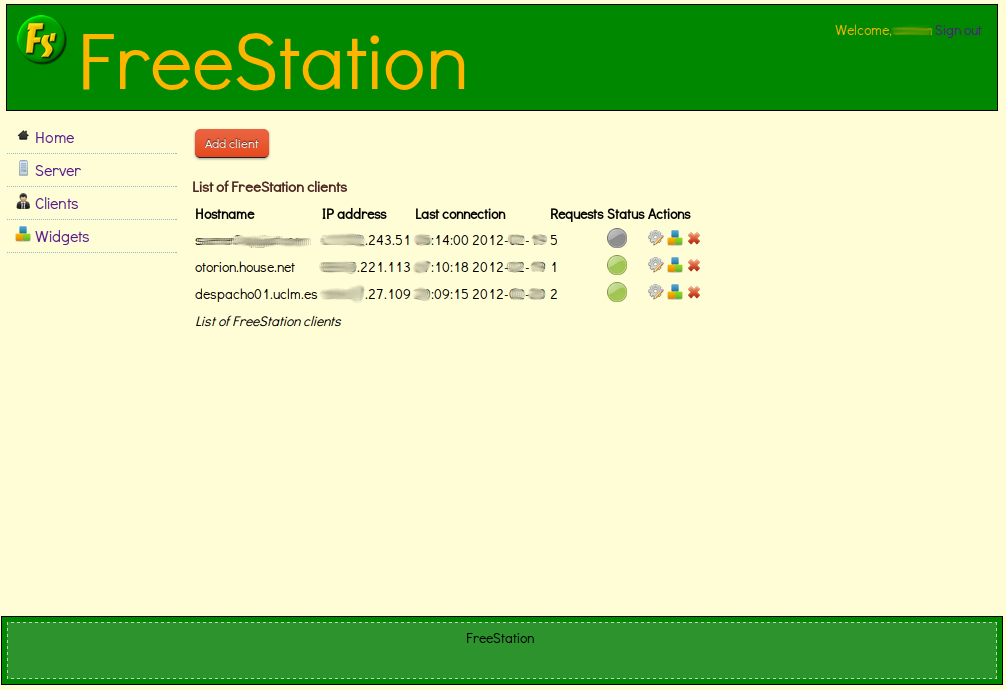
\includegraphics[width=300px]{src/img/freestation-server-clients.png}
            \caption[Listado de clientes]
              {Listado de clientes}
             \label{fig:listclients}
        \end{center}
    \end{figure}
    
    \newpage
    Para añadir o autorizar un cliente se debe ingresar al sistema
    autentificando con los credenciales de usuario y contraseña. Posteriormente
    acceder a la sección ``Clients`` como se muestra en la figura
    ~\ref{fig:listclients} y pulsar sobre el botón ``Add client``.

    Después, rellenar con los datos del cliente (IP, hostname) y estado.
    
    \begin{figure}[ht]
        \begin{center}
            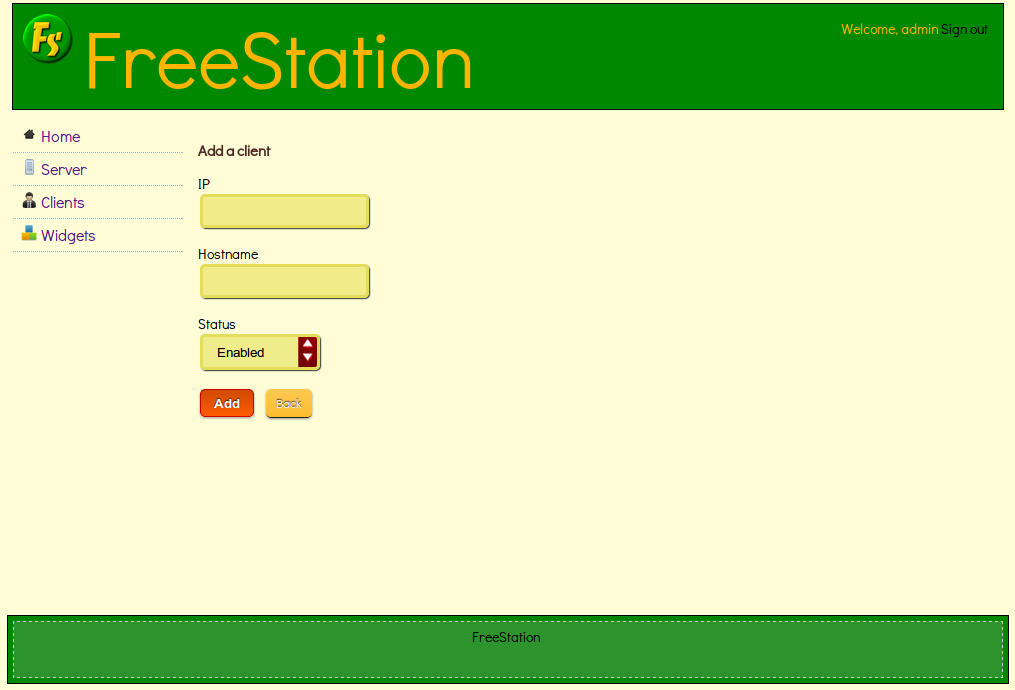
\includegraphics[width=300px]{src/img/add-client.png}
            \caption[Añadir cliente FreeStation]
              {Añadir cliente FreeStation}
        \end{center}
    \end{figure}
    
    \subsection{Como deshabilitar un cliente}
    
    La vista de estaciones freestation de la figura  ~\ref{fig:listclients},
    indica un listado de servidores y clientes activos/suspendidos.
    
    Pulsando sobre el icono de circulo verde puede deshabilitarse un cliente o
    bien habilitarse si el icono del círculo es gris.
    
    También puede editarse el estado pulsando sobre el icono de engranaje.
    
    \subsection{Como añadir un widget a un cliente}
    
    El \emph{Frontend} dispone de una vista de widgets por servidor, donde
    pueden ser activados/desactivados además de acceder a sus 
    parametrizaciones correspondientes.
    
    \newpage
    
    \begin{figure}[ht]
        \begin{center}
            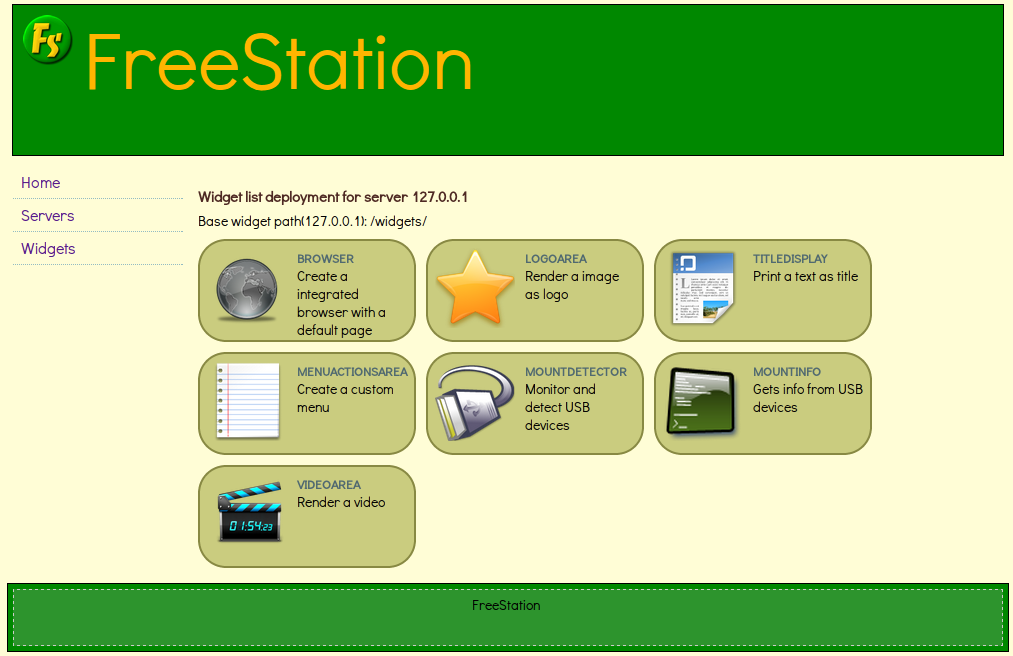
\includegraphics[width=300px]{src/img/widget_view.png}
            \caption[Vista de Widgets]
              {Vista de Widgets}
        \end{center}
    \end{figure}
    
    Pulsando sobre el icono de widgets en la vista cliente como se muestra en la
    figura ~\ref{fig:listclients} se accede a un listado de los widgets
    disponibles para dicho cliente.
        
    Posteriormente pueden asociarse nuevos widgets pulsando sobre el botón
    ``Associate'' y eligiendo en la lista de disponibles:
    
    \begin{figure}[ht]
        \begin{center}
            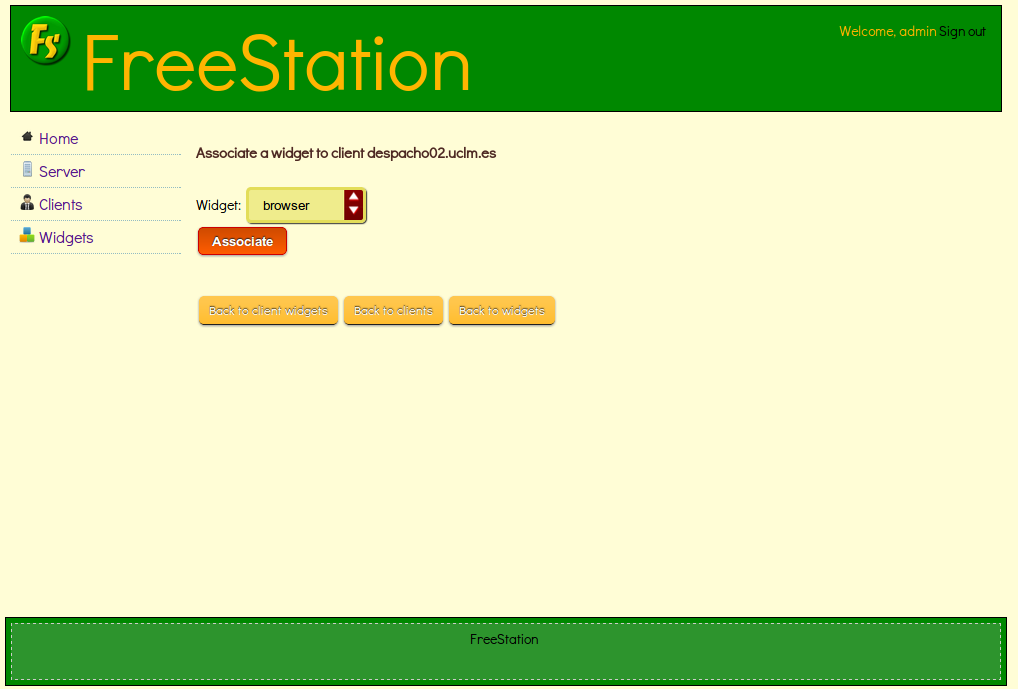
\includegraphics[width=300px]{src/img/associate-widget-client.png}
            \caption[Asociar un widget para un cliente]
              {Asociar un widget para un cliente}
        \end{center}
    \end{figure}
    
    Dependiendo de la implementación del widget, puede ser editado para ese
    cliente ofreciendo la configuración personalizada.
    
    \begin{figure}[ht]
        \begin{center}
            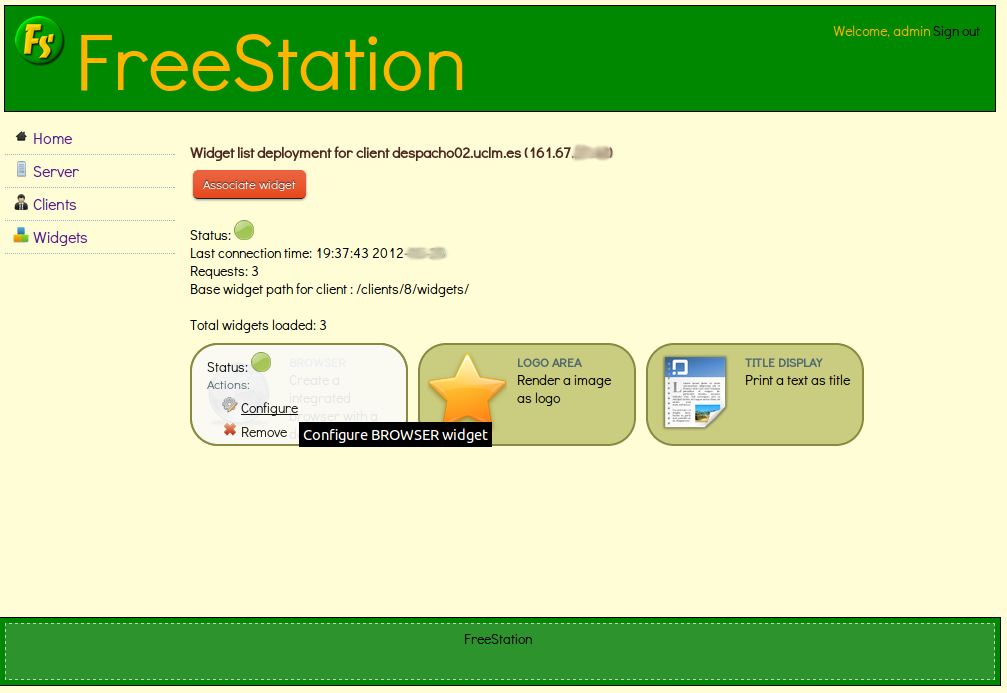
\includegraphics[width=300px]{src/img/configure-widget-client.png}
            \caption[Configurar widget para un cliente]
              {Configurar widget para un cliente}
        \end{center}
    \end{figure}
    
    \newpage
    En este caso, el widget Browser muestra la personalización del título y url
    a cargar:
    
   \begin{figure}[ht]
        \begin{center}
            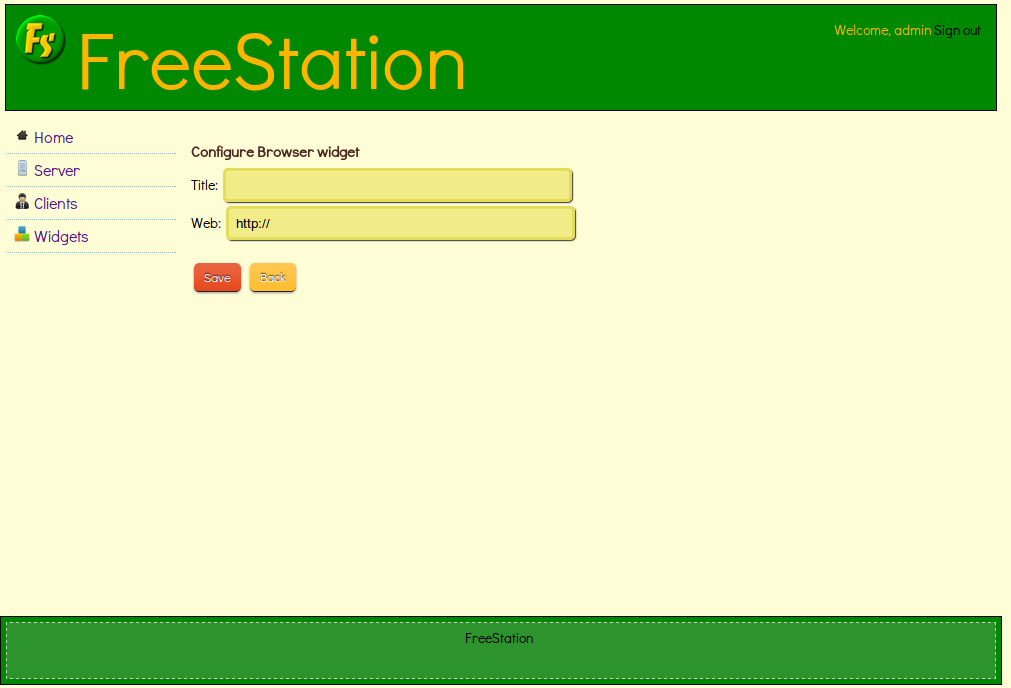
\includegraphics[width=300px]{src/img/configure-widget-browser.png}
            \caption[Configurar widget Browser]
              {Configurar widget Browser}
        \end{center}
    \end{figure}
    
    \subsection{Como añadir nuevos widgets al servidor}
    
    En la sección widgets del servidor aparece un listado de los disponibles.
    
    \newpage
    
    \begin{figure}[ht]
        \begin{center}
            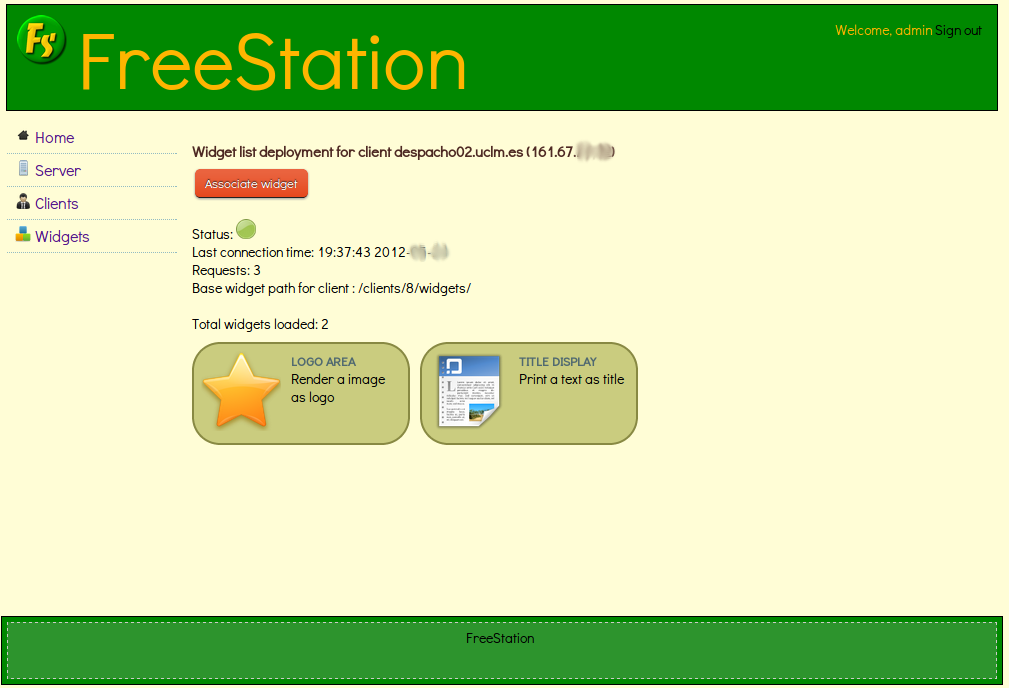
\includegraphics[width=300px]{src/img/widget-for-client.png}
            \caption[Lista de widgets para un cliente]
              {Lista de widgets para un cliente}
        \end{center}
    \end{figure}
    
    Pulsando sobre el botón ``Add widget'' se procederá a una lectura del
    directorio de widgets para búsqueda de nuevos widgets. Para ello, el
    widget debe estar implementado en el \emph{Frontend} para su uso.
    
    \subsection{Como administrar el servidor desde \emph{Frontend}}
    
    Para iniciar o parar o incluso reiniciar el servidor desde \emph{Frontend}
    se debe hacer click en la sección ``Server''. Después el icono de círculo
    verde o gris mostrará el estado de encendido o apagado respectivamente.
    
    \newpage
    
    \begin{figure}[h]
        \begin{center}
            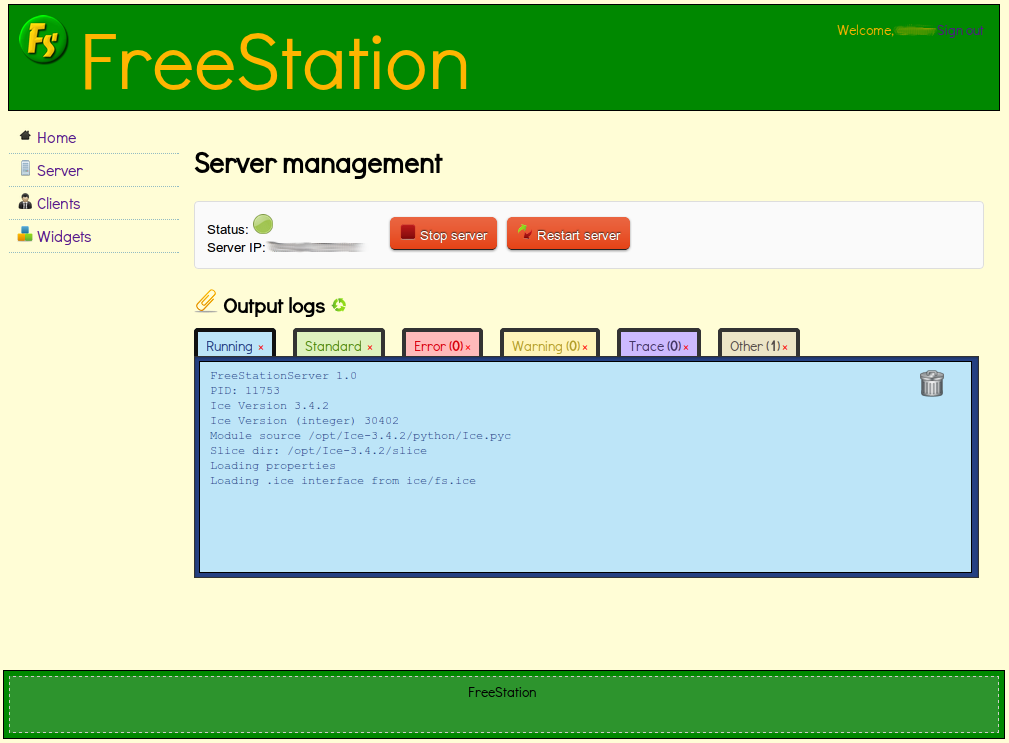
\includegraphics[width=300px]{src/img/freestation-server-gui.png}
            \caption[FreeStation Server Webserver GUI] {FreeStation Server Webserver GUI}
            \label{fig:serverGUI}
        \end{center}
    \end{figure}

    Según sea el estado se podrá apagar o reiniciar o iniciar. En las pestañas
    de logs puede visualizarse la información relevante de conexiones y
    peticiones de los clientes o fallos si se producen.
    
    %%sudo apt-get install openjdk-6-jre
    %%sudo dpkg -i openproj\_1.4-2.deb
    
    %%sudo apt-get install cloc
    
    \cleardoublepage


    \chapter{Apéndice C: Código fuente}
    
    Debido a la extensión del código fuente de \emph{FreeStation}, éste se
    incluye únicamente en su versión electrónica en el CD adjunto a este documento.
    
    \section{\uppercase{Instalación del entorno servidor}}
    
    La estructura de directorios con la que se ha organizado este código fuente es la siguiente:

    Para el entorno cliente:
    \textbf{fs}
    
    \begin{itemize}
      \item freestation: el directorio que contiene la mayor parte del
      desarrollo del cliente, este contiene directorios útiles como:
          \begin{itemize}
              \item files: espacio donde se almacenan los archivos descargados
              para copias de USB
              \item ice: almacena los slices para Zero C ICE.
              \item img: guarda los recursos de imágenes utilizados en el
              cliente.
              \item ogv: guarda los vídeos utilizados en el cliente en formato
              ogv
              \item templates: plantillas HTML para el widget Browser.
              \item test: contiene los test unitarios realizados sobre el
              cliente.
              \item themes: pruebas de themes para GTK.
              \item ui: contiene la interfaz para el caso de explotación basado
              en CouchDB
              \item widgets: almacena los widgets basados en GTK disponibles
              para el cliente
              \item xml: guarda las configuraciones de widgets para el cliente.
            \end{itemize}
      \item test: conteine los test generales realizados sobre pruebas de
      concepto.
    \end{itemize}
    
    Para el entorno servidor:
    \textbf{freestation-web}
    \begin{itemize}
      \item backend: almacena los ficheros de \emph{Backend}, slices, api y
      módulo FS de Zero C ICe.
      \item css: almacena los archivos css del \emph{Frontend}.
      \item docs: este directoriose ha generado autodocumentación con sphinx
      como prueba desde el código python. La versión de esta documentación no esta completa pero
      puede ser orientativa. Puede accederse online desde:
      \url{http://freestation.quijost.com/docs/\_build/}
      \item img: contiene las imágenes del \emph{Frontend}.
      \item inc: incluye los archivos de cabeceras y pie de página para el CMS.
      \item js: bibliotecas de javascript utilizadas.
      \item lib: contiene las clases principales del CMS.
      \item sql: guarda una copia del SQL generado en la primera instalación.
      \item test: test en PHP.
      \item tmp: directorio temporal.
      \item widgets: widgets configurados.
    \end{itemize}
    
    \cleardoublepage
    %% Free Documentation License
    %\blankpage
    %\part{Apéndice}
    
% Local Variables:
% coding: utf-8
% mode: latex
% TeX-master: "main"
% mode: flyspell
% ispell-local-dictionary: "castellano8"
% End: